Where previously I added an optical potential to the Hamiltonian for a short time during the evolution, here I directly engineer the wavefunction phase. For the previously chosen kicking strengths and timestep, the limiting values of the phase change are $\approx 0.2 < \phi < \approx 0.94$. This is determined by writing the phase as
\begin{equation}
    e^{i\phi} \mapsto e^{-i\frac{V_\textrm{opt}dt}{\hbar}},
\end{equation}
and filling in for the defined simulation values. Thus, for a much stronger phase change a longer lasting pulse, or a greater amplitude are two possible contenders. However, as discussed previously, neither are suitable candidates in this system, given the lattice rotation, as well as the excitation of higher-order wavenumbers. With the use of direct phase imprinting we can realise arbitrary phase patterns on the condensate. Previously the vortex lattice was unaffected by the imprint; here I attempt to destroy the vortex lattice by directly engineering the opposite phase winding profile atop a lattice vortex. This has the distinct advantage of locally erasing a vortex and disordering the lattice. I will now discuss this method.

\section{Model}



As previously discussed, to investigate the evolution of a perturbed vortex lattice I numerically solve the Gross--Pitaevskii equation in two dimensions, assuming a strong confinement along the third axis. This allows to restrict the dynamics to the $x$--$y$ plane and focus fully on the Abrikosov lattice geometry. Experimental setups in lower dimensions are currently available \cite{BEC:Stock_lpl_2004,BEC:Seo_jkps_2014,BEC:Chomaz_natcom_2015} and in the frame co-rotating with the condensate, the non-linear mean field equation governing the BEC wave-function is given by
\begin{align}
i\hbar\partial_t \Psi(\mathbf{r},t) = \Big[&-\frac{\hbar^2}{2m}\nabla^2 + V\left(\mathbf{x}\right) \nonumber\\
&+ g\vert \Psi(\mathbf{r},t) \vert^2- \Omega L_z \Big]\Psi(\mathbf{r},t),
\end{align}
which is the previously used form as given by \ref{eqn:gpe2d}.
Here $V\left(\mathbf{x}\right)$ is the trapping geometry, $\Omega$ is the trap rotation frequency, and $L_z$ is the angular momentum operator along the $z$-direction. For the rapidly rotating case, the vortices form an ordered triangular lattice, that rotates equivalently to a solid-body in the large number limit. Deviations from the solid-body rotation can be seen for trajectories in the limit of long times ($\approx 10$ s). This is very likely due to long-wavelength Tkachenko modes in the condensate, and following the analysis of \cite{BEC:Baym_prl_2003} has a frequency much longer than the lifetime of the system for our given rotation rate.
%However, due to the density inhomogeneities of a harmonically trapped condensate, and the likelihood of shearing this is (I think) expected.
The lattice is well ordered and behaved at timescales on the order of up to several seconds, as well as away from the condensate edges, and so we
will restrict our analysis therein.

As condensates are highly controllable in the lab \cite{BEC:Fetter_rmp_2009}, I consider the use of many common experimental techniques to engineer specific states otherwise difficult in solid-state materials. One such set of systems are those of two-dimensional crystals with controllable defects, which although (relatively) easily created classically \cite{XTAL:Bragg_prsa_1947,OPT:Kim_spie_2011}, are difficult experimentally in quantum systems due to the sizes of interatomic spacings. Here we propose the use of phase-imprinting \cite{Vtx:Dobrek_pra_1999} as a means of achieving such defects in a vortex lattice of a Bose-Einstein condensate. Through direct manipulation of the condensate phase, vortices may be added or removed from specific locations in the system.

%%%%%%%%%%%%%%%%%%%%%%%%%%%%%%%%%%%%%%%%%%%%%%%%%%%%%%%%%%%%%%%%%%%%%%%%%%%%%%%%%%%%%%%%%%%%%%%%%%%%%%%%%%%%%%%%%%%%%%%%%%%%%%%%%%%%%%%%%%%%%
%\subsection{Order/disorder}
%%%%%%%%%%%%%%%%%%%%%%%%%%%%%%%%%%%%%%%%%%%%%%%%%%%%%%%%%%%%%%%%%%%%%%%%%%%%%%%%%%%%%%%%%%%%%%%%%%%%%%%%%%%%%%%%%%%%%%%%%%%%%%%%%%%%%%%%%%%%%
%Given the localised defect disturbs the lattice after sufficiently long times, we can examine if the lattice moves from global ordered to
%disordered following the addition or removal of another site over the course of time. For a two-dimensional material, KTHNY theory describes
%the transitions from a solid crystalline to amorphous fluid phase, via an intermediate hexatic phase. This state is generally characterised
%by the translational and orientational correlation functions long-ranged behaviour. As we have an inhomogeneous density profile, and a system with a %finite size, the use of translational correlations does not make much sense. Orientational correlations however, which
%measure how the lattice aligns along a particular angle, should suffice when combined with the density structure factor,
%$S = \int d\mathbf{r}e^{i\mathbf{k}\cdot\mathbf{r}}|\Psi|^2$. True crystaline behaviour is given by a constant orientational value, with
%power-law decay expected for a hexatic phase, and exponential decay for an amorphous fluid (neglecting translational correlations).

%%%%%%%%%%%%%%%%%%%%%%%%%%%%%%%%%%%%%%%%%%%%%%%%%%%%%%%%%%%%%%%%%%%%%%%%%%%%%%%%%%%%%%%%%%%%%%%%%%%%%%%%%%%%%%%%%%%%%%%%%%%%%%%%%%%%%%%%%%%%%
\subsection{Phase imprinting defects}
%%%%%%%%%%%%%%%%%%%%%%%%%%%%%%%%%%%%%%%%%%%%%%%%%%%%%%%%%%%%%%%%%%%%%%%%%%%%%%%%%%%%%%%%%%%%%%%%%%%%%%%%%%%%%%%%%%%%%%%%%%%%%%%%%%%%%%%%%%%%%
Phase imprinting is a technique that applies a spatially inhomogeneous optical potential across a condensate in such a way that the phase is modified to a desired form. As a consequence the density distribution will adjust itself and in ground state condensates dark solitons \cite{BEC:Denschlag_science_2000}, as well as vortices have been created this way \cite{Vtx:Dobrek_pra_1999}. For the latter the signature is given by a phase singularity, around which the phase winds through $\pm 2\pi$, depending upon the direction of rotation.

However, the phase imprinting method can also be used to eliminate a vortex from the lattice by applying a phase profile of opposite winding that eliminates the phase singularity.  This will leave the condensate with a density depletion at the prior location of the phase singularity. However, since the singularity is no longer present, this depletion will fill in and excite phonon modes in the condensate. Since phonons have been shown to yield minimal impact on the vortex lattice structure \cite{VTX:Oriordan_pra_2016}, we can safely ignore their contribution. The removal of a vortex from the lattice introduces a vacancy to the system.


\lee{The energy hierarchy upon goes as
\[ E_{1centre} < E_{1centre-d} < E_{2-1} < E_{2} \]
with a change of
\begin{align} E_{1centre-d} - E_{1centre} \approx 1 \\
 E_{2-1} - E_{1centre} \approx 1.5 \\
 E_{2} - E_{1centre} \approx 1.9 \\
E_{2-1} - E_{1centre-d} \approx 0.5 \\
E_{2} - E_{2-1} \approx 0.4
\end{align}
all in units of $\hbar \Omega$, where $\Omega = 0.25*\omega_{\perp}$.
}





\section{Vortex dynamics}\label{sec:vtxdyn}
\subsection{Single vortex in a BEC}
To fully understand the effect of removing a vortex from the lattice system, I will first investigate the effects from removing the vorticity from a single vortex carrying condensate. The results of this process can be seen in Fig.~\ref{fig:annihilation_1vtx}, and, as expected, the depletion of the condensate density fills in after the vortex phase is removed. This creates a sound wave, which expands outwards at a rate given by the local speed of sound in the condensate, before rebounding again inwards, and continuing this oscillation process.
\begin{figure}
    %\includegraphics[width=0.45\textwidth]{imgs/1vtx_phaseimp}%{imgs/EKspec/Density_1kill}
    \includegraphics[width=0.45\textwidth]{imgs/NEWPICS/1vtx_remove1_centred}
%    \includegraphics[width=0.45\textwidth]{tikz/graph_r2}

    \caption{The evolution of the condensate density (top) and phase (bottom) is shown for the initial state, and after 10 ms of evolution. As can be seen, the density ripples expand radially outwards. }\label{fig:annihilation_1vtx}
\end{figure}

\begin{figure}
    \includegraphics[width=0.45\textwidth]{tikz/graph_r2}
    \caption{The breathing mode frequency of the condensate following the imprint is shown here, and matches the expected value of $2\omega_\perp$.}\label{fig:breathing}
\end{figure}


\begin{figure}
    \includegraphics[width=0.45\textwidth]{imgs/1vtx_remove1_uncentred}%{imgs/EKspec/Density_1kill}
    \caption{The condensate evolution following an uncentered phase imprint. For an imprint that is of the order of the healing length from centre to centre, the annihilation occurs during the evolution (a,b). However, beyond this distance, we create an antivortex which causes motion of the pre-existing positive vortex (c,d,e).}\label{fig:annihilation_1vtx_uncentred}
\end{figure}
\begin{figure}[tb]
    \includegraphics[width=0.35\textwidth]{tikz/EKt}
    %\includegraphics[width=0.35\textwidth]{imgs/EKspec/EK_0}
    %\includegraphics[width=0.35\textwidth]{imgs/EKspec/EK_100}
    %\includegraphics[width=0.3\textwidth]{imgs/EKspec/EK_1000}
    %\includegraphics[width=0.3\textwidth]{imgs/EKspec/EK_3000}
    \caption{Compressible kinetic energy spectrum at times $t=0$ (solid) and $t=\tau$ (dashed), where $\tau=10$ ms.
    Initially the incompressible energy is greater than the compressible due to the presence of a vortex. After application of the phase profile, the vortex is annihilated, with the energy released as phonons, which is indicated by the increase in compressible, and decrease of incompressible energy.}
\end{figure}



\begin{figure}[bt]
\includegraphics[width=0.3\textwidth]{imgs/EKspec/EK_6000}
\includegraphics[width=0.3\textwidth]{imgs/EKspec/EK_8000}
\includegraphics[width=0.3\textwidth]{imgs/EKspec/EK_10000}
\includegraphics[width=0.3\textwidth]{imgs/EKspec/EK_100000}
    \caption{Compressible kinetic energy spectrum at times (T to B) 60ms, 80ms, 100ms, 1s.}
\end{figure}

It can be noted that during the initial expansion, subsequent contractions and oscillations, interference rings are observed in the density. These can also be observed in the quantum compressible [cite anderson paper] energy spectra, and can be seen to show periodic occurrence (see Fig. \ref{fig:qucomp_1vtxann}). This is expected, as annihilation event creates local density oscillations which in turn emit phonons in the BEC, which expand radially outwards from the point of origin.


\begin{figure}\label{fig:qucomp_1vtxann}
    \includegraphics[width=0.48\textwidth]{imgs/EKspec/EKc_cl}
    \includegraphics[width=0.48\textwidth]{imgs/EKspec/EKc_qu}
    \caption{Compressible kinetic energy over time after removing a single vortex. Classical and quantum (with phase during calculation) cases are given.}
\end{figure}

An examination of the squared-radial expectation value, $\langle r^2 \rangle$, where $r^2 = x^2 + y^2$, shows that removing the vortex from the condensate excites a breathing mode, at the expected frequency of $2\omega_\perp$ for a two-dimensional system (see Fig. \ref{fig:r2_breathing}). If

In addition to the ideal situation of perfect erasing of a perfectly centred vortex discussed above, two additional situations are of interest. The first is when the erasing phase is not centred on the phase singularity (see Fig.~\ref{fig:annihilation_1vtx_uncentred}). As one can see
for cases where the imprinted profile is sufficiently close to the core (i.e. within the healing length), the two annihilate as before. However, beyond this distance the vortex-antivortex pair travel to the edge of the condensate system, and begin to circulate around, as expected. The phonons released by the creation of the antivortex remains centred on the point of application, and spreads outwards, as seen with the annihilation case. Therefore, one can see there are three phonon generation process; the creation of the antivortex within the bulk density, the annihilation of the vortex by direct application of the phase, and the pair annihilation by vortex-antivortex collision, when sufficiently close.


The second question to ask is what happens to other vortices that are in the vicinity of the one to be erased. For this in Fig.~\ref{fig:2k1} I show a simulation where one vortex is erased in a two vortex condensate. Since the size of the vortex cores are on the order of the healing length, and therefore small compared to any other length-scale in the system, one can see that the other vortex just experiences a constant shift in energy and its vorticity is not affected. This is even more true in a situation where the vortices are closer together.


\begin{figure}
    \includegraphics[width=0.48\textwidth]{imgs/EKspec/2kill1_traj}
    \caption{The two vortex condensate before annihilating one vortex. The trajectory of the second vortex is superimposed, showing that the induced phonons have no effect on the path of the vortex, which circulates at a different rate due in the corotating frame due to the loss of one quantum of angular momentum.}\label{fig:2k1}
\end{figure}

\section{Order/disorder in vortex lattices}\label{sec:disorder}
%%%%%%%%%%%%%%%%%%%%%%%%%%%%%%%%%%%%%%%%%%%%%%%%%%%%%%%%%%%%%%%%%%%%%%%%%%%%%%%%%%%%%%%%%%%%%%%%%%%%%%%%%%%%%%%%%%%%%%%%%%%%%%%%%%%%%%%%%%%%%

I represent the vortex lattice as a graph, where each vortex is treated as a node, with edges given by nearest neighbours at most separated by a distance $a_0$, for a triangular lattice configuration, or $\sqrt{2}a_0$ for a square lattice (see Fig. \ref{fig:vtxdist}). The inclusion of the square lattice distance is chosen so that upon removal, the vortices can reconfigure their arrangement locally, and may move from triangular to square geometries. As they behave like Coulombic particles with a profile that falls off as $r^{-1}$ we can consider that any interactions outside these distances to be negligible.

According to KTHNY theory for a 2D material the transition from an ordered solid crystal to a liquid phase is mediated through an intermediary hexatic phase. This state is generally characterised by the translational and orientational correlation functions long-ranged behaviour. In the following I will first study the effect of the removal of a single vortex from a vortex lattice, and then later increase the number of removed vortices, and examine the impact on the vortex lattice order. Given that the localised defect disturbs the lattice after sufficiently long times, we can examine if the lattice moves from a global ordered to disordered state following an addition or removal event, and if the system follows a solid-hexatic-amorphous phase transition.

As we have an inhomogeneous density profile, and a system with a finite size, the use of translational correlations does not make much sense. Orientational correlations however, which measure how the lattice aligns along a particular angle, as well as pair correlations may be useful. To quantify the disturbance created, we calculate the orientational correlation function given by
\begin{equation}\label{eqn:g6r}
	g_6(r) = \frac{1}{N(r)}\displaystyle\sum\limits_{i,j}^{N(r)}\psi_6(\mathbf{r}_i)\psi_6^{*}(\mathbf{r}_j),
\end{equation}
with
\begin{equation}\label{eqn:psi6r}
	\psi_6(|\mathbf{r}_{i} - \mathbf{r}_{j}|) = \frac{1}{n_i}\displaystyle\sum\limits_j^{n_i}\exp(6\mathrm{i}(\theta_i - \theta_j)),
\end{equation}
where $\psi_6$ is the orientational order parameter, and $j$ is over the nearest neighbouring vortices, as well as the pair correlation function, $g(r)$, given by
\begin{equation}\label{eqn:gr}
	g(r_k) = \frac{1}{A_k}\left\langle \displaystyle\sum\limits_{i}\displaystyle\sum\limits_{j\neq i}\delta(r-r_{ij}) \right\rangle
\end{equation}
where $i,j$ are respective indices of individual vortices, $k$ identifies the bin shell radius, $r_{ij}=|\mathbf{r}_i - \mathbf{r}_j|$, $A_k$ is the shell area, and $\langle \rangle$ is the ensemble average. Instead of the translational correlation function, $g_T(r)$, commonly used as a measure of order in KTHNY theory, we instead opt for the density structure factor $S = \int d\mathbf{r}e^{i\mathbf{k}\cdot\mathbf{r}}|\Psi|^2$, delaunay triangulation, and voronoi tessellation of the vortex lattice system. Although we cannot draw quantitative results from the pair correlation function, one can qualitatively see how crystalline the material is by the sharpness of the peaks, especially when combined with the structure factor, $S(\mathbf{k})$. True crystalline behaviour is given by a constant orientational correlation value, with power-law decay expected for a hexatic phase, and exponential decay for an amorphous fluid (neglecting translational correlations).

Here I examine the orientational correlation function as a measure of the order of a ``vortex unit cell'', consisting of the angle made by nearest neighbours to an individual vortex. For a perfectly ordered triangular lattice this value will tend to 1. To maintain constant vortex areal density, I have chosen vortices defined at a radius of $r=2\times 10^{-4}$ m from the centre, which give an almost uniform lattice constant for our system parameters. Following the description given by \cite{Nelson_pma_1982}, crystalline order is indicated by a non-zero orientational correlation, and well defined structure factor peaks, with hexatic phases indicated by arithmetic decay of the correlations and smeared structure factor peaks. For amorphous materials, the correlations follow an exponential decay, with the Fourier shells indicating the lack of crystalline behaviour in the structure factor. Here I examine such behaviour.


%%%%%%%%%%%%%%%%%%%%%%%%%%%%%%%%%%%%%%%%%%%%%%%%%%%%%%%%%%%%%%%%%%%%%%%%%%%%%%%%%%%%%%%%%%%%%%%%%%%%%%%%%%%%%%%%%%%%%%%%%%%%%%%%%%%%%%%%%%%%%

\subsection{Lattice vacancy}
%%%%%%%%%%%%%%%%%%%%%%%%%%%%%%%%%%%%%%%%%%%%%%%%%%%%%%%%%%%%%%%%%%%%%%%%%%%%%%%%%%%%%%%%%%%%%%%%%%%%%%%%%%%%%%%%%%%%%%%%%%%%%%%%%%%%%%%%%%%%%
The removal of a single vortex from the vortex lattice is thus expected to affect only the nearest neighbours by altering their velocity well, with the overall angular momentum of the condensate decremented by a single quantum. The resulting vacancy, following a vortex removal, remains localised to its respective position within the lattice for long times, regardless of initial placement (assuming not at the edge) (see Fig. \ref{fig:trajectory}). The resulting stability of the nearest neighbours follows a decay of the honeycomb-like structure akin to that described by \cite{Vtx:Leipold_jsm_2016}. Given enough time, this structure decays via one of the three possible means, creating a locally disordered region. However, even for long times, the overall vortex lattice remains well structured, as evidenced by examining correlation functions of the vortex positions for both pair, and orientational correlations.

\include{g6rimg}

To examine the vortex dynamics following the application of the phase profile, each individual vortex is tracked independently. We can observe the local effects of disturbing the lattice by examining the Delaunay triangulation and Voronoi tessellation of the vortex lattice. We perform this by first creating the Delaunay triangulation of the lattice. Next, using the resulting triangulation the edges are bisected, and the bisectors lengthening until they intersect with other bisectors. The lines terminate at these points of contact, and the resulting structure is the voronoi tessellation of the data. %This is a useful method to visualise periodicity and order of a set of data, given the orientation and size of the resulting cells.



Delaunay trianuglation is useful as a means to indicating the locations of disclinations (non 6-fold connected edges) in the lattice.  An alternative view is given by the Voronoi tessellation, which can be used to indicate the value of arbitrary quantities in  different regions of the lattice.

Here we make use of these methods to visualise the order of the vortex lattice upon phase imprinting. The delaunay triangulation of the lattice upon removing a single vortex is given in Fig.~\ref{fig:deltri_1vtx}. A pair of 5 and 7-fold disclinations can be considered as a lattice dislocation, and can be seen to remain localised for long times following a vortex removal. The voronoi diagram Fig.~\ref{fig:voronoi_100ms} similarly demonstrates the localisation of the topological defect, with the color of each cell given by its area, dicated by inter-vortex spacings. After the vortex removal, the system maintains the topological defect for lines times, after which the vortices begin to deviate from their lattice positions and attempt to fill the vacancy and balance
the inter-vortex forces. The long-time behaviour is shown by Fig.~\ref{fig:voronoi_1vtx}, indicating both lattice density (cell area) and local orientational order.



\begin{figure}[bt]
    \includegraphics[width=0.48\textwidth]{./imgs/NEWPICS/delaunay_varr161.pdf}
    \caption{Delaunay triangulation of vortex lattice after removing 1 vortex, viewed at $t=\{0,0.01,0.8,4,6,10\}$ s. A pair of 5-7 dislocations persists in the lattice into long times.}\label{fig:deltri_1vtx}
\end{figure}

\begin{figure}[tb]
	\includegraphics[width=0.48\textwidth]{imgs/Disloc_-1_centre_avgarea}
	\caption{Voronoi cell average area after removing vortex at condensate centre. \tb{This plot currently does not really say anything. What does it mean that the average size oscillates? Later you say that nothing is happening until about 100ms, so we should zoom in around that time.}}
	\label{fig:voronoi_area}
\end{figure}

Removing vortices at different positions in the lattice shows similar behaviour, with the effect on the velocity profile and trajectories of other vortices being mostly localised around the removal site.

%\iffalse
\begin{figure}[tb]
	\includegraphics[width=0.48\textwidth]{imgs/Disloc_-1_centre_voronoi_t100ms_cbar}
	\caption{Voronoi cells after removing vortex at condensate centre for t=100 ms. Vortices at edge boundary neglected. }
	\label{fig:voronoi_100ms}
\end{figure}
%\fi

\begin{figure}[tb]
    \includegraphics[width=0.48\textwidth]{./imgs/NEWPICS/varr161/voronoi_area/voronoi_999000}
    \includegraphics[width=0.48\textwidth]{./imgs/NEWPICS/varr161/voronoi_colour/voronoi_999000}
    \caption{Voronoi diagram of cell area and local orientational order after removing 1 vortex, viewed at $t=10$ s.}\label{fig:voronoi_1vtx}
\end{figure}


Tracking the vortex distances traveled for different removal locations, and for a different number of removed vortices shows how much we
disturb the underlying lattice (see \ref{fig:vtxdist}).

\begin{figure}[tb]
	\includegraphics[width=0.48\textwidth]{imgs/vtx_distance_travelled}
	\caption{Vortex total traveled distance with different removal positions for between 1 and 3 vortices.}
	\label{fig:vtxdist}
\end{figure}


\subsubsection{Lattice overpopulation}
%%%%%%%%%%%%%%%%%%%%%%%%%%%%%%%%%%%%%%%%%%%%%%%%%%%%%%%%%%%%%%%%%%%%%%%%%%%%%%%%%%%%%%%%%%%%%%%%%%%%%%%%%%%%%%%%%%%%%%%%%%%%%%%%%%%%%%%%%%%%%
Similarly to removing a vortex from the lattice, we can also add one. By choosing a pre-existing vortex and adding a like-signed phase
winding, we can create multiply charged vortices in the condensate, where the vortex has a winding of $2\pi l$, with $l$ as the vortex
charge. Multiply charged vortices are usually unstable in condensates, as it is more energetically favourable to have two singly charged
vortices, than a single doubly charged vortex, as the energy increases with $l^2$. Thus, an $l$-charged vortex is expected to instead decay
into $l$ singly-charged vortices.

Here we have taken our lattice of $l=1$ vortices, and given an additional charge to a single vortex to examine the decay process. However,
the presence of the lattice suppresses the decay process for long times (order of seconds) compared to that of in a condensate without vortex
lattice. The doubly charged vortex remains stable on the order of seconds even away from the lattice centre (though does decay eventually).
The additional velocity profile locally causes the nearest neighbouring vortices to rotate faster than the solid-body rotation rate of the
whole lattice, causing a local shearing of the lattice structure. As with the vacancies, the use of correlation functions allowed us to
examine the short and long-range order of the lattice.

Voronoi diagrams of the resulting lattice show a stable doubly charged vortex position, with show twisting of the lattice about this central
point.

\begin{figure}[tb]
	\includegraphics[width=0.49\textwidth]{imgs/DoubleCharge/add161/voronoi}
	\includegraphics[width=0.49\textwidth]{imgs/DoubleCharge/add161remove207/voronoi}
	\caption{(top) Doubly charged central vortex. Doubly charged vortex remains stable, and retains 6-fold
	symmetry of vortex lattice. (bottom) Doubly charged central vortex, and removal of nearby vortex. Doubly charged vortex remains stable, and forms 8-fold
	symmetry of vortex neighbours.}
	\label{fig:voronoi_double}
\end{figure}


%%%%%%%%%%%%%%%%%%%%%%%%%%%%%%%%%%%%%%%%%%%%%%%%%%%%%%%%%%%%%%%%%%%%%%%%%%%%%%%%%%%%%%%%%%%%%%%%%%%%%%%%%%%%%%%%%%%%%%%%%%%%%%%%%%%%%%%%%%%%%
\subsection{Things to note}
%%%%%%%%%%%%%%%%%%%%%%%%%%%%%%%%%%%%%%%%%%%%%%%%%%%%%%%%%%%%%%%%%%%%%%%%%%%%%%%%%%%%%%%%%%%%%%%%%%%%%%%%%%%%%%%%%%%%%%%%%%%%%%%%%%%%%%%%%%%%%

\begin{itemize}
\item Localised disturbances: introducing vacancy to lattice causes it to travel with lattice. Change in velocity profile only affects 6
nearest neighbours on moderate timescales.
\item Long range hexatic phase has short range translational order (exp drop off), but constant orientational order -> is this such a phase?
\end{itemize}

%%%%%%%%%%%%%%%%%%%%%%%%%%%%%%%%%%%%%%%%%%%%%%%%%%%%%%%%%%%%%%%%%%%%%%%%%%%%%%%%%%%%%%%%%%%%%%%%%%%%%%%%%%%%%%%%%%%%%%%%%%%%%%%%%%%%%%%%%%%%%
\subsection{Correlations}
%%%%%%%%%%%%%%%%%%%%%%%%%%%%%%%%%%%%%%%%%%%%%%%%%%%%%%%%%%%%%%%%%%%%%%%%%%%%%%%%%%%%%%%%%%%%%%%%%%%%%%%%%%%%%%%%%%%%%%%%%%%%%%%%%%%%%%%%%%%%%



%%%%%%%%%%%%%%%%%%%%%%%%%%%%%%%%%%%%%%%%%%%%%%%%%%%%%%%%%%%%%%%%%%%%%%%%%%%%%%%%%%%%%%%%%%%%%%%%%%%%%%%%%%%%%%%%%%%%%%%%%%%%%%%%%%%%%%%%%%%%%
\subsection{Numerics and analytics}\label{sec:numerics}
%%%%%%%%%%%%%%%%%%%%%%%%%%%%%%%%%%%%%%%%%%%%%%%%%%%%%%%%%%%%%%%%%%%%%%%%%%%%%%%%%%%%%%%%%%%%%%%%%%%%%%%%%%%%%%%%%%%%%%%%%%%%%%%%%%%%%%%%%%%%%

Each vortex position was found by summing over adjacent grid sites, and looking for a $2\pi$ phase winding. This gave a vortex position
estimated to the numerical grid. A least-squares fit was performed to more accurately determine the vortex core. Vortices closest the centre
of the condensate were considered to ensure an almost uniform inter-vortex spacing, giving minimal deviation in lattice constant, $a_0$. Each
vortex was assigned a unique identifier (UID) to allow for it to be tracked individually over the course of the simulations, with the initial
configuration presented in the graph [ref graph]. By noting these UIDs, vortices can be individually selected for removal by applying the
global $2\pi$ phase winding in the opposing direction, centered on the core.

The trajectory plots show very small global effect on the core positions, with a disturbance localised in a region centered on the removed
core. By removing vortices in different locations on the condensate we see similar behaviour, with the trajectories modified in a region
around the removed vortex. The removal of two vortex adjacent cores can be seen to crate a greater disturbance, as expected, with the
trajectories of the surrounding vortices no longer following an almost circular path (more like hexagonal), but taking on other geometric
path shapes. For two nn vortices the path becomes an almost rhombic shape, with nnn forming an elongated hexagon (as to be expected). For 3
nn, the resulting trajectories follow a triangular pattern of the same orientation as the removed vortices. For the removal of an entire 7
vortex cell, the formed pattern is star shaped.

TODO:
Calculate incompressible kinetic energy spectrum for each case, and see if useful. RESULT: It wasn't.
Calculate $S(k) = |\Psi(k)|^2$ for condensate densities, not just vortex positions, for comparison. RESULT: looks strange, even in untouched
case. Arcs exist in all cases, but with interference lines.

The impact on the overall distances traveled by each vortex as a result of the dislocations is given in figure [some fig].

\begin{figure}[tb]
	\includegraphics[width=0.48\textwidth]{imgs/mono}
	\caption{The oscillation of the mean-radius of the condensate after the addition of vortices (positive) or antivortices (negative) with
	different imprinted windings. The oscillation mode shows an exact match for a 2D non-rotating condensate of $2\omega_{\perp}$ for all cases.}
\end{figure}


\begin{figure}[bt]
	\includegraphics[width=0.48\textwidth]{imgs/FFT_density_linear_cell}
	\caption{Density structure factor within 4*pi/(sqrt(3)*d0).}
\end{figure}



\begin{figure}[htb]
	\includegraphics[width=0.48\textwidth]{imgs/FFT_density}
	\caption{Density structure factor.}
\end{figure}


\begin{figure}[tb]
	\includegraphics[width=0.48\textwidth]{imgs/RDF_time_gp}
	\caption{Radial distribution function over time after removing vortex from lattice centre. }
\end{figure}


\begin{figure}[tb]
	\includegraphics[width=0.48\textwidth]{imgs/graph86}
	\caption{Condensates vortices treated as nodes in a graph. Edges are drawn between nearest neighbours.}
\end{figure}
%\fi

%%%%%%%%
%%%%%%%%



\begin{figure}[htb]
    \includegraphics[width=0.48\textwidth]{./imgs/NEWPICS/varr161anti/voronoi_area/voronoi_999000}
    \includegraphics[width=0.48\textwidth]{./imgs/NEWPICS/varr161anti/voronoi_colour/voronoi_999000}
    \caption{Voronoi diagram of cell area and local orientational order after replacing 1 vortex with an antivortex, viewed at $t=10$ s.}
\end{figure}
\begin{figure}[htb]
    \includegraphics[width=0.48\textwidth]{./imgs/NEWPICS/varrnuclear/voronoi_area/voronoi_999000}
    \includegraphics[width=0.48\textwidth]{./imgs/NEWPICS/varrnuclear/voronoi_colour/voronoi_999000}
    \caption{Voronoi diagram of cell area and local orientational order after removing 7 vortices, viewed at $t=10$ s.}
\end{figure}
\begin{figure}[htb]
    \includegraphics[width=0.48\textwidth]{./imgs/NEWPICS/varr161/g6rT}
    \includegraphics[width=0.48\textwidth]{./imgs/NEWPICS/varr161/grT}
    \caption{Figure shows the orientational (T) and radial (B) correlation functions over time as a function of distance for removing a single vortex.}
\end{figure}
\begin{figure}[htb]
    \includegraphics[width=0.48\textwidth]{./imgs/NEWPICS/varr161anti/g6rT}
    \includegraphics[width=0.48\textwidth]{./imgs/NEWPICS/varr161anti/grT}
    \caption{Figure shows the orientational (T) and radial (B) correlation functions over time as a function of distance for adding an anti vortex.}
\end{figure}
\begin{figure}[htb]
    \includegraphics[width=0.48\textwidth]{./imgs/NEWPICS/varrnuclear/g6rT}
    \includegraphics[width=0.48\textwidth]{./imgs/NEWPICS/varrnuclear/grT_caxis1}
    \caption{Figure shows the orientational (T) and radial (B) correlation functions over time as a function of distance for removing 7 vortices.}
\end{figure}
\begin{figure}[htb]
    \includegraphics[width=0.48\textwidth]{./imgs/NEWPICS/varr161/traj_10s}
    \includegraphics[width=0.48\textwidth]{./imgs/NEWPICS/varr161anti/traj_10s}
    \includegraphics[width=0.48\textwidth]{./imgs/NEWPICS/varrnuclear/traj_10s}
    \caption{Trajectory plots for removing 1, removing and adding an antivortex, and removing 7 vortices for 10 s of time [\lee{can be made much shorter too.}]}
\end{figure}
\begin{figure}[htb]
    \includegraphics[width=0.48\textwidth]{./imgs/NEWPICS/varrnuclear/EKc_cl_log_1_250}
    \includegraphics[width=0.48\textwidth]{./imgs/NEWPICS/varrnuclear/EKi_cl_log_1_250}
    \caption{Classical compressible and incompressible kinetic energy spectra after removal of 7 vortices in log scale.}
\end{figure}
\begin{figure}[h!tb]
    \includegraphics[width=0.48\textwidth]{./imgs/NEWPICS/varrnuclear/EKc_qu_nonlog_1_250}
    \includegraphics[width=0.48\textwidth]{./imgs/NEWPICS/varrnuclear/EKi_qu_nonlog_1_250}
    \caption{Quantum compressible and incompressible kinetic energy spectra after removal of 7 vortices in linear scale.}
\end{figure}
\begin{figure}[htb]
    \includegraphics[width=0.48\textwidth]{./tikz/graph_rv}
    \caption{The average intervortex spacing after introducing a lattice defect. Plots are shown for removing 1, removing and adding an antivortex, and removing 7 vortices.}
\end{figure}
%%%%%%%%




%%%%%%%%%%%%%%%%%%%%%%%%%%%%%%%%%%%%%%%%%%%%%%%%%%%%%%%%%%%%%%%%%%%%%%%%%%%%%%%%%%%%%%%%%%%%%%%%%%%%%%%%%%%%%%%%%%%%%%%%%%%%%%%%%%%%%%%%%%%%%
\section{Conclusions}\label{sec:conc}
%%%%%%%%%%%%%%%%%%%%%%%%%%%%%%%%%%%%%%%%%%%%%%%%%%%%%%%%%%%%%%%%%%%%%%%%%%%%%%%%%%%%%%%%%%%%%%%%%%%%%%%%%%%%%%%%%%%%%%%%%%%%%%%%%%%%%%%%%%%%%

The removal of a vortex from the lattice creates a stable vacancy site, which in the corotating frame, travels with the lattice for some time
before decaying into paired 5 and 7 nearest neighbour disclinations. These disclination pairs can be viewed as as an edge dislocation in the
lattice. The resulting grain boundary breaks the 6-fold symmetry of the triangular lattice. The removal of the single vortex also removes the
velocity profile associated with the vortex at that location. The local velocity near the vacancy will be less than the solid-body behaviour
of the lattice. This causes the nearest neighbour vortices to rotate slower than the condensate, locally creating a strain/shear? on the
lattice. Local competition to fill the vacancy ensures its long-lived stability. The removal of the central vortex creates a local honeycomb
lattice structure, which according to [stat top of 2d lattice] will decay (following perturbation) via three possible processes.

Increasing the charge of a vortex by applying the same signed phase winding to a vortex core creates a stable doubly charged vortex for long
times (seconds). This, like the stable vacancy, seems to be stable at any range of positions (but decays faster at outskirts). The additional
velocity field shears the lattice, with the resulting correlations showing long-range power-law behaviour. This is usually indicative of a
power-law hexatic phase. Given the lack of true translational order in a harmonically trapped vortex lattice, it remains more instructive to
investigate the static structure factor of the system. The hexatic phase is expected to show spreading of the Fourier peaks into arcs. Here,
though we see such spreading, it is not entirely arc-like, and does not match entirely with the expectations of a hexatic phase.
